\section{Complexity Considerations} \label{sec:complexity}
% ================================================================================

%In this section, we calculate estimates for the maximal number of test
%executions to be performed when testing for failures refinement
%and---as a corollary---trace refinement.
%Theorem~\ref{th:failurestest} specifies that all tests $U_F(j),\ 0\le j < pq$
%need to be executed, where $p$ denotes the number of nodes in the transition
%graph of the reference process $P$, and $q\ge p$ is an estimate for the
%maximal number of nodes in the SUT's transition graph. Therefore, we will first
%calculate a bound for the number of test executions to be performed for test
%$U_F(j)$ and then summarise  these bounds over all $j$ from $0$ to $pq-1$.
%
%For the worst-case estimate, we first introduce a CSP reference process $\pmax$
%which
%turns out to be--given a fixed alphabet $\Sigma$---the test
%model leading to the maximal number
%of test executions for every $U_F(j)$ when considering large alphabets. In the case
%of small alphabets and large values of $pq-1$, it will turn out below that a variant
%of $\pmax$ will lead to the maximal number of executions. The conditions for this
%can also be clearly specified.

%we assume that $P$ never allows for early
%deadlock (so $\minhits(P/s)$ is never empty) and that the SUT $Q$ is a
%correct failures refinement. Therefore, all test executions
%$(Q\parallel[\Sigma] U_F(j))$ stop after having run through a trace of $Q$ of
%length $j+1$, because their is no early termination due to entering branches
%(\ref{eq:ufa}), (\ref{eq:ufb}), or due to an illegal deadlock of $Q$. As can
%be seen from the specification of the test cases $U_F(j)$ (see
%Section~\ref{sec:finitecompletefails}), the number of executions ending in a
%$\epass$ event corresponds to the number $\ell$ of traces $s$ of $P$ with
%length equal to $j$, multiplied by the number $h$ of minimal hitting sets in
%$\minhits(P/s)$. For the tests $U_T(j)$ verifying trace refinement (see
%Section~\ref{sec:finitecomplete}), the number of executions equals $\ell$,
%since there is no equivalent in $U_T(j)$ to checking different hitting sets
%in the last step of a test execution. \fixme{But doesn't this add to the
%number of executions?} \fxnote{jp: should be clear now from the revised test}

Since we have finite complete CSP test suites, it is useful for the first
time to calculate how many test executions are needed when using them.
Previous work did not consider sufficient conditions for finiteness, so
complexity was not a concern. We answer the following questions. (1)~What is
the worst-case bound on the number of test executions to be performed to
verify an SUT with respect to failures refinement, when we use our test
suite? (2)~What is the worst-case bound for trace refinement? (3)~Is it
possible to reduce the maximal length of traces when testing for failures or
trace refinement? We consider the first question~(1) in
Section~\ref{section:complexity:failures}), where we also discuss whether it
it is possible to reduce the number of test executions with a different test
suite.  With the answer to question~(1), question~(2) is a fairly simple
consequence we discuss briefly also in
Section~\ref{section:complexity:failures}. Question~(3) is the subject of
Section~\ref{section:complexity:length}.

% -------------------------------------------------------------------------
\subsection{Estimates for the Maximal Number of Failures Test Executions}
\label{section:complexity:failures}

An arbitrary CSP process $P$ might have $\minhits(P/s) = \varnothing$ for
some traces $s$, so that a test case $U_F(j)$ for a $j$ greater than the size
of $s$ can enter branch~(\ref{eq:ufb}). In this case, further executions are
needed to consider traces that have $s$ as a prefix.  To provide a bound on
the number of test executions needed, we first define a process $\pmax$~(see
(\ref{eq:pmax})), which, when used as a reference process, requires the
maximal number of test executions among all reference processes $P$
fulfilling $\minhits(P/s) \neq \varnothing$ for all traces $s$. For $\pmax$,
we can establish the actual number of test executions required~(see
(\ref{eq:pmaxcomplexity})). We then show that the order of magnitude of the
worst-case bound for the number of test executions is the same also for
reference processes $P$ that may have $\minhits(P/s) = \varnothing$ for some
$s$.

% -----------------------------------------------------------------------------
\paragraph{A Reference Process} Given an alphabet $\Sigma$ of size $\card{\Sigma} =
n\ge 2$, define a collection of subsets of $\Sigma$ by
\begin{equation}\label{eq:defC}
  {\cal C} = \{ A\subseteq\Sigma~|~\card{A} = n - \lfloor\frac{n}{2}\rfloor + 1 \}.
\end{equation}
%
With this choice of ${\cal C}$, define
\begin{equation}\label{eq:pmax}
  \pmax = \Intchoice_{A\in{\cal C}} e:A\then \pmax
\end{equation}
%
The relevant properties of $\pmax$ are summarised in the following lemma.
%
\begin{lemma}\label{lemma:pmax}
  Given alphabet $\Sigma$ with cardinality $\card{\Sigma} = n\ge 2$,
  process $\pmax$ fulfils
  %
  \begin{eqnarray}
  {}[\pmax/s]^0 & = & \Sigma \quad\text{for all $s\in \Sigma^*$}
  \label{eq:pmaxa}
  \\
  \trc(\pmax) & = & \Sigma^*
  \label{eq:pmaxb}
  \\
  \minaccs(P/s) & = & {\cal C} \quad\text{for all $s\in \Sigma^*$}
  \label{eq:pmaxc}
  \\
  \minhits(P/s) & = & \minhits({\cal C}) \quad\text{for all $s\in \Sigma^*$}
  \label{eq:pmaxe}
  \\
  \card{\minhits(P/s)} & = & \binom{n}{\lfloor\frac{n}{2}\rfloor}
  \quad \text{for all $s\in \Sigma^*$}
  \label{eq:pmaxd}
  \\
  \minhits({\cal C})  & = & \{ H\subseteq \Sigma~|~\card{H} = \lfloor\frac{n}{2}\rfloor\}
  \label{eq:pmaxf}
  \end{eqnarray}
\end{lemma}
\begin{proof}
Since $\bigcup_{A\in{\cal C}} A = \Sigma $ by construction of ${\cal C}$,
$[\pmax/s]^0 = \Sigma$ as stated by (\ref{eq:pmaxa}). Since $\pmax/e = \pmax$
for all $e\in\Sigma$, this proves statement (\ref{eq:pmaxb}). The internal
choice construct used in the specification of $\pmax$ implies
$\minaccs(\pmax) = {\cal C}$. Again, $\pmax/e = \pmax$ for all $e\in\Sigma$
implies $\minaccs(\pmax/s) = {\cal C}$ for all traces of $\pmax$, so this
shows (\ref{eq:pmaxc}). Statement (\ref{eq:pmaxe}) is a direct consequence of
(\ref{eq:pmaxc}). Let $H$ be any minimal hitting set of ${\cal C}$. Then $H$
contains at least $\lfloor{\frac{n}{2}}\rfloor$ elements, because otherwise
$\card{\Sigma\setminus H} > n-\lfloor{\frac{n}{2}}\rfloor$, and any subset
$A\subseteq \Sigma\setminus H$ with cardinality
$n-\lfloor{\frac{n}{2}}\rfloor+1$  would be contained in ${\cal C}$, but
satisfy $A\cap H=\varnothing$. Since
$\lfloor{\frac{n}{2}}\rfloor+n-\lfloor{\frac{n}{2}}\rfloor+1=n+1$, we
conclude that any $\lfloor{\frac{n}{2}}\rfloor$-element subset of $\Sigma$
intersects  every element of ${\cal C}$.  Therefore, every minimal hitting
set of ${\cal C}$ has exactly $\lfloor{\frac{n}{2}}\rfloor$ elements; this
shows (\ref{eq:pmaxf}) and $\card{\minhits({\cal C})} =
\binom{n}{\lfloor{\frac{n}{2}}\rfloor}$. The latter shows  (\ref{eq:pmaxd})
and completes the proof. \xbox
\end{proof}

% -----------------------------------------------------------------------------
\paragraph{Test Cases of $\pmax$} The test cases $U_F(j)$ generated from $\pmax$ can
never enter branch (\ref{eq:ufa}), because $\pmax/s$ has initials $\Sigma$
for all traces $s\in\trc(\pmax)$ according to (\ref{eq:pmaxa}). Moreover,
they can never enter branch (\ref{eq:ufb}), because $\minhits(\pmax/s)$ is
never empty according to (\ref{eq:pmaxd}). Finally, the minimal hitting sets
used to probe the SUT at the end of a non-blocking test execution are always
the hitting sets of ${\cal C}$ according to (\ref{eq:pmaxe}). This results in
the following test case structure.
\begin{eqnarray*}
\label{eq:UFPpmax}
U_F(j) & = & U_F(j,0,\ii n)
\\
U_F(j,k,n) & = &   (k < j) \& \big(e:\Sigma   \then U_F(j,k+1,t(n,e) \big)
\\ & & \extchoice
\\ & & (k = j) \& \big( \Intchoice_{H\in\minhits({\cal C})} (e:H   \then \epass \then\Stop   )  \big)
\end{eqnarray*}
This means that the branches of $U_F(j)$ that can lead to an early
termination are not feasible. All tests deadlock, or run to the end of a
trace of size $j$ and then present a choice of events from a minimal hitting
set.

Moreover, Theorem~\ref{th:sperner} establishes that given an alphabet with
$n$ elements, there is no Sperner family consisting of more than
$\binom{n}{\lfloor\frac{n}{2}\rfloor}$. In addition, we recall the minimal
hitting sets calculated from a given set of minimal acceptances are a Sperner
family~(see discussion in Section~\ref{sec:sperner}). So, (\ref{eq:pmaxd})
establishes that there is no possibility of providing more choices fom
minimal hitting sets with a test derived from a process different from
$\pmax$.

In summary, the tests derived from $\pmax$ require the most test executions
when compared to tests derived from any other CSP process $P$ whose
collections of minimal hitting sets $\minhits(P/s)$ are never empty for any
trace $s$.

% -----------------------------------------------------------------------------
\paragraph{Maximal Number of Test Executions for $\pmax$}
When considering the number of test executions to be performed using $U_F(j)$
derived from $\pmax$ against some SUT $Q$ for all $j = 0,\dots,pq-1$, and
considering that we need to cover all the possible behaviours of $Q$, the
maximal number of test executions is only reached if (a)~$Q$ is a correct
refinement of $\pmax$ (or more generally, of the reference process) and
(b)~its traces are $\Sigma^*$.
%or if it fails in the very last execution of the very last $U_F(j)$
%executed against $Q$. If an erroneous behaviour of $Q$ is revealed before
%this very last execution, the test experiment is stopped (and $Q$ can be
%fixed before executing the suite again). Therefore, we consider only correct
%SUTs $Q$ when determining the maximal number of executions that can be
%executed.
%
%For the  $U_F(j)$ generated from $\pmax$, the number of test executions
% to be performed is maximal if $\pmax\lessdet_F Q$ and
%$\trc(Q) = \Sigma^*$.
In such a situation, no test execution blocks early, because $Q/s$ can always
engage into some $e\in\Sigma$  while $\#s<j$, and never blocks in the last
step when $\#s = j$ and a hitting set $H\in\minhits({\cal C})$ is offered by
the test case. The resulting number of executions in this case is
%
\begin{equation}
\label{eq:maxexec}
n^{j}\cdot \binom{n}{\lfloor\frac{n}{2}\rfloor},
\end{equation}
%
because all traces up to length $j$ can be executed with $U_F(j)$
entering branch (\ref{eq:ufc}), and each of these traces is followed by one
event from each of the hitting sets of ${\cal C}$ since $Q$ is correct.  %(b) leads to the maximal number of
%executions possible, because it is responsible for the factor *n^{(pq-1)} in
%the upper bound (47), (48) [n = |Sigma|]. Considering a reference process
%with fewer traces or an implementation Q with fewer traces would
%significantly reduce the value of this factor, while just adding one
%additional execution possibility for branch (20), after which the test suite
%is stopped due to failure.

The number of executions in (\ref{eq:maxexec}) is indeed maximal for all
reference processes $P$ fulfilling $\minhits(P/s)\neq\varnothing$ for all
traces $s$. All these processes can never enter branch (\ref{eq:ufb}), and,
if an execution with an SUT entered branch (\ref{eq:ufa}), this would only
lead to early termination of the whole test suite, because a failure has been
detected. As a consequence, $\card{\Sigma}^{j}$ is the maximal number of
traces to be executed up to length $j$, and from Theorem~\ref{th:sperner} we
know that the number $\binom{n}{\lfloor\frac{n}{2}\rfloor}$ of hitting sets
to be tested at the end of each trace of length $j$ is already maximal.

Summing up  formula (\ref{eq:maxexec}) over all test cases
$U_F(0),\dots,U_F(pq-1)$ to be executed and applying the formula for the sum
of a geometric progression,  this results int
%
\begin{equation}\label{eq:pmaxcomplexity}
\sum_{j=0}^{pq-1} n^{j}\cdot \binom{n}{\lfloor\frac{n}{2}\rfloor}  =
\binom{n}{\lfloor\frac{n}{2}\rfloor}\cdot\frac{1-n^{pq}}{1-n}\quad\text{with $n=\card{\Sigma}$}
\end{equation}
%
as the maximal number of test executions to be performed when testing an
error-free SUT $Q$ with $\trc(Q) = \Sigma^*$ against the reference process
$\pmax$. If we are interested only in the order of magnitude, we have
%
\begin{equation}
\label{eq:maxO}
O\big(\binom{n}{\lfloor\frac{n}{2}\rfloor}\cdot n^{pq-1}\big)\quad\text{with $n=\card{\Sigma}$}.
\end{equation}

% -----------------------------------------------------------------------------
\paragraph{Considering Empty Collections of Minimal Hitting Sets}
The argument so far has shown that the tests derived from $\pmax$ require the
most test executions when considering processes whose collections of minimal
hitting sets are never empty. %Lemma~\ref{lemma:failureshittingsets} implies
%that an empty collection $\minhits(P/s)$ is equivalent to $(s,A)\in\fails(P)$
%for all $A\subseteq\Sigma$. This is equivalent to $\maxrefs(P/s) = \{ \Sigma
%\}$ or $\minaccs(P/s) = \{ \varnothing\}$.
%
It remains to consider whether reference processes $Z$ possessing failures
$(s,\Sigma)$ may require more test executions for their associated tests
$U_F(j)$ than the bound given for $\pmax$ in (\ref{eq:pmaxcomplexity}),
because process states $Z/s$ with $\minhits(Z/s)=\varnothing$ allow for test
executions entering branch (\ref{eq:ufb}). To this end, consider a test case
$U_F(j)$ constructed from such a process $Z$. Every trace $s\in\trc(Z)$ with
$\#s<j$ ending in a process state $Z/s$ with $\minhits(Z/s)=\varnothing$
allows for
%
\begin{itemize}
\item one execution of branch (\ref{eq:ufb}), where the test execution
$(Z\parallel[\Sigma]U_F(j))/s$ stops after $\epass$, and
\item $\card{[Z/s]^0}$   continuations of the test execution with events $e\in [Z/s]^0$.
\end{itemize}
%
For every trace $s\in\trc(Z)$ with $\#s=j$,
%
\begin{itemize}
\item one execution of branch (\ref{eq:ufb}) follows if
$\minhits(Z/s)=\varnothing$, and otherwise
\item $\card{\minhits(Z/s)}$ executions checking acceptance of minimal hitting sets.
\end{itemize}
%
For a rough estimate of the worst-case upper bound suppose that
%
\begin{enumerate}
\item $[Z/s]^0 = \Sigma$ for all traces $s$ of $Z$,
\item all traces $s$ with $\#s<j$ end in a state with empty minimal hitting sets, and
\item all traces $s$ with $\#s=j$ end in a state with a maximal number $\binom{n}{\lfloor n/2\rfloor}$
 of hitting sets.
\end{enumerate}
%
We note that this scenario is not feasible for all $j\in\{0,\dots,pq-1\}$,
because the traces of $U_F(p-1)$ already cover all states of $Z$'s transition
graph according to Lemma~\ref{lemma:extendV}, and if all states of $Z$ have
empty hitting sets, there are no acceptance checks to be performed in the
last step of the test execution. Therefore, \pagebreak the upper bound
calculated next cannot be reached by a CSP process. With the three
assumptions above, nevertheless, we can calculate that
%
\begin{itemize}
\item  $U_F(0)$ has  $\binom{n}{\lfloor n/2\rfloor}$ executions,
\item $U_F(j)$, for $j > 0$ has $\sum_{i=0}^{j-1} n^i = \frac{n^j -
    1}{n-1}$ executions of branch (\ref{eq:ufb}), ($n = \card{\Sigma}$),
    and
\item $U_F(j)$, for $j > 0$ has $\binom{n}{\lfloor n/2\rfloor}\cdot n^j$
    executions where the acceptance of hitting sets is checked after having
    run through a trace of length $j$.
\end{itemize}
%
Summing up over all $U_F(j)$ for $j=0,\dots,pq-1$, an upper bound $B$ may be calculated as follows.
%
\begin{eqnarray*}
B & = & \binom{n}{\lfloor n/2\rfloor} + \sum_{j=1}^{pq-1} \frac{n^j - 1}{n-1} +
\sum_{j=1}^{pq-1}\binom{n}{\lfloor n/2\rfloor}\cdot n^j
   \\
& = &    \sum_{j=1}^{pq-1} \frac{n^j - 1}{n-1} +
\sum_{j=0}^{pq-1}\binom{n}{\lfloor n/2\rfloor}\cdot n^j
\\
& = & \frac{n^{pq}-n pq+pq-1}{(n-1)^2} +
\binom{n}{\lfloor n/2\rfloor} \cdot \frac{n^{pq} - 1}{n-1}
\\
& = &
\\
& = & \frac{\binom{n}{\left\lfloor \frac{n}{2}\right\rfloor}(n-1) \left(n^{pq}-1\right) +n^{pq}-npq+pq-1}{(n-1)^2}
\end{eqnarray*}
%
Since $B$ cannot be reached anyway, we just calculate its order of magnitude,
and this results again in $O\big(\binom{n}{\lfloor\frac{n}{2}\rfloor}  \cdot
n^{pq-1}\big)$, as calculated already for $\pmax$ in (\ref{eq:maxO}).
%
Summarising these complexity calculations, we have the following theorem.
%
\begin{theorem}
\label{th:maxexecs}
Given a process alphabet $\Sigma$, consider a fault model ${\cal F} = (P,\lessdet_F,{\cal D})$, such that
the normalised transition graph of $P$ has $p$ states, and the fault domain
${\cal D}$ contains all processes $Q$ over alphabet $\Sigma$, such that $G(Q)$ has at most
$q\ge p$ states. Then the maximal
number of test executions to be performed   using the complete test
suite $\TS_F = \{ U_F(j)~|~0 \le j < pq  \}$ created from $P$ as specified in Theorem~\ref{th:failurestest} is of order
%
\begin{equation*}
O\big(\binom{n}{\lfloor\frac{n}{2}\rfloor}\cdot n^{pq-1}\big)\quad\text{with $n=\card{\Sigma}$}.
\end{equation*}
For processes $P$ satisfying $(s,\Sigma)\not\in\fails(P)$ for all traces $s$, the reachable
precise  upper bound is given by
%
\begin{equation*}
\binom{n}{\lfloor\frac{n}{2}\rfloor}\cdot\frac{1-n^{pq}}{1-n}\quad\text{with $n=\card{\Sigma}$}.
\end{equation*}
\xbox
\end{theorem}
%
As established by Lemma~\ref{lemma:hseta}, the number of hitting sets used to
probe the SUT cannot be reduced:~if the reference process is $\pmax$, we need
to consider all of them, otherwise illegal blocking may remain undetected. In
addition, if $\pmax$ defines the behaviour of the SUT, using smaller sets
that are no longer hitting sets lead to a rejection of correct
implementations. Our explicit definition of $\pmax$ to establish this
worst-case is useful to illustrate this point.

In~\cite{Hennessy:1988:ATP:50497}, it is suggested to test {\it every}
non-empty subset of $\Sigma$ whose events cannot be completely refused in a
given process state of the reference model; this leads to a worst-case
estimate of $2^{\card{\Sigma}}-1$ for the number of different sets to be
offered to the SUT in the last step of the test execution. This number is
significantly larger than the worst-case estimate $\binom{n}{\lfloor
n/2\rfloor}$ above. In Fig.~\ref{fig:minhita}, the reduction is visualised by
plots of the two functions. In~\cite{DBLP:conf/icfem/CavalcantiG07}, the
authors also use minimal hitting sets\footnote{However, they are denoted by
{\it minimal acceptances} in~\cite{DBLP:conf/icfem/CavalcantiG07}.}, but do
not give an estimate for the number of test executions.

% .....................................................................................
 \begin{figure}
 %%\hspace*{-40mm}
 \begin{center}
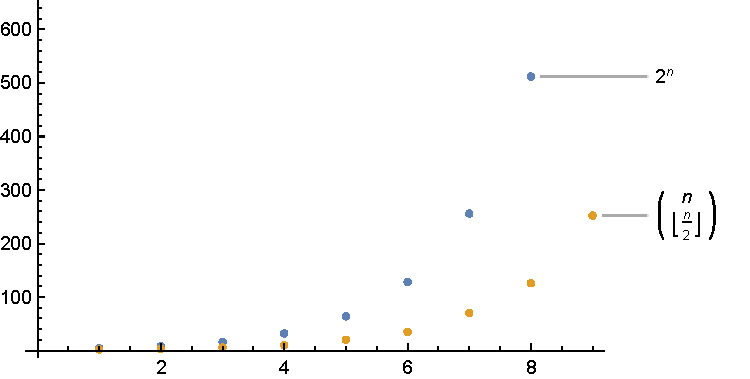
\includegraphics[scale=.7%width=.8\textwidth
                        ]{curvecomparison.pdf}
\end{center}
%\vspace*{-10mm}
\caption{Function plot $2^{\card{\Sigma}}$ versus $\binom{n}{\lfloor \frac{n}{2}\rfloor}$.}
 \label{fig:minhita}
 \end{figure}
% .......................................................................................

% -------------------------------------------------------------------------
\paragraph{Estimate for the Maximal Number of Trace Test Executions}
%\label{section:complexity:traces}
According to Theorem~\ref{th:tracetest}, a complete test suite checking trace
refinement just contains the adaptive test case $U_T(pq-1)$. As derived for
$U_F(j)$ above, the maximal number of executions to be performed by
$(Q\parallel[\Sigma] U_T(pq-1))$ is of order
$O\big(\card{\Sigma}^{pq-1}\big)$.

% -------------------------------------------------------------------------
\subsection{Upper Bound $pq$ for the Maximal Length of Test Traces}
\label{section:complexity:length}

According to Theorem~\ref{th:failurestest}, the tests $U_F(j)$ need to be
executed for $j = 0,\dots,pq-1$ to guarantee completeness. So, the SUT is
verified with test traces up to, and including, length $pq$. With branch
(\ref{eq:ufa}), $U_F(j)$ accepts all traces $s.e$ with $s\in\trc(P), \#s
= j, e\not\in\trc(P/s)$, so erroneous traces up to length $j+1$ are detected.

It is interesting to investigate whether this maximal length is necessary, or
one could elaborate alternative complete test strategies where the
SUT is tested with shorter traces only. Indeed, an example
in~\cite[Exercise~5]{PeleskaHuangLectureNotesMBT} shows that, when testing
for equivalence of deterministic FSMs, it is sufficient to test with
traces of significantly shorter length.

The following example, however, shows that the maximal length $pq$ is really
required when testing for refinement.
%\begin{example}\label{ex:pq}
%Consider the CSP reference process $P$ and an erroneous implementation $Q$
%specified as follows.
%
%\begin{center}
%\begin{minipage}{.4\textwidth}
%\begin{eqnarray*}
%P & = & a \then P_1 \intchoice b \then P_1 \intchoice c \then P_1
%\\
%P_1 & = & a \then P \extchoice b\then P
%\end{eqnarray*}
%\end{minipage}
%\hfill
%\begin{minipage}{.4\textwidth}
%\begin{eqnarray*}
%Q & = & a\then Q_1 \extchoice b\then Q_1
%\\
%Q_1 & = & a\then Q_2 \extchoice b\then Q_2
%\\
%Q_2 & = & a\then Q \intchoice b\then Q
%\end{eqnarray*}
%\end{minipage}
%\end{center}
%
%
%\medskip
%Obviously, $P$'s normalised transition graph has 2 nodes, while $Q$'s graph
%has 3. It is easy to see (and can be checked with FDR4) that $P\lessdet_T Q$,
%but $\neg(P\lessdet_F Q)$. Furthermore, it can also be shown using FDR4 that
%the ``test passed condition''
%\[
%(\epass\then\Stop) \lessdet_F (Q\parallel[\Sigma] U_F(j))\hide \Sigma
%\]
%holds for $U_F(0),\dots,U_F(4)$, but fails for $U_F(5)$. So, the
%non-conformance of $Q$ cannot be detected by any test trace of length less or
%equal to 5, but is revealed (as expected from Theorem~\ref{th:failurestest})
%by a trace of length 6, because the last event offered by the test $U_F(5)$
%is refused by $Q$. \xbox
%\end{example}

\begin{example}\label{ex:pq}
Consider the CSP reference process $P$ and an erroneous implementation $Q$
specified as follows.
%
\begin{eqnarray*}
P & = &  P(0)
\\
P(k) & = & (k < p-1) \& \big( (a \then P(k)) \intchoice ( b \then P(k+1))\big)
\\ & & \extchoice
\\ & & (k = p-1) \& (a \then P(k))
\\
Q & = & Q(0)
\\
Q(k) & = & (k < q-1) \& \big( a \then Q(k+1)    \big)
\\ & & \extchoice
\\ & & ( k = q-1)\& \big( a\then Q(0) \extchoice b\then Q(0)  \big)
\end{eqnarray*}
%
The normalised transition graphs of $P$ and $Q$ are depicted in
Fig.~\ref{fig:examplepq} for the case $p=3,\ q=4$. Using FDR4, it can be
shown for concrete values of $p$ and $q$ that the  ``test passed conditions''
\[
(\epass\then\Stop) \lessdet_F (Q\parallel[\Sigma] U_F(j))\hide \Sigma
\quad
\mathrm{and}
\quad
(\epass\then\Stop) \lessdet_T (Q\parallel[\Sigma] U_T(j))\hide \Sigma
\]
hold for $j = 0,\dots,pq-2$. So, none of the test cases $U_F(j)$ and $U_T(j)$
are capable of detecting failures and trace refinement violations, if they
only check traces up to length $pq-1$. (We recall that this corresponds to
$j\le pq-2$).

$Q$, however, neither conforms to $P$ in the failures refinement relation,
nor in the trace refinement relation. This can only be seen when executing
the test $U_F(pq-1)$ and $U_T(pq-1)$, respectively. These tests fail, so this
shows that $P\not\lessdet_F Q$ and $P\not\lessdet_T Q$ according to
Theorem~\ref{th:failurestest} and Theorem~\ref{th:tracetest}. Moreover, this
shows that the maximal trace length $pq$ to be investigated in the tests
cannot be further reduced without losing the completeness property of the
test suites. \xbox
\end{example}
%
Generalising Example~\ref{ex:pq}, it can be shown that for any $p,q \geq 2$,
%\in\mathbb{N}$,
there exist reference processes $P$ with $p$ states and
implementation processes $Q$ with $q$ states, such that a violation of the
trace refinement property can only be detected with a trace of length $pq$.
This is proven in the following
theorem. %In the proof, we use the processes $P$ and $Q$ introduced in Example~\ref{ex:pq}.

\begin{figure}[tbp]
\begin{center}
\begin{minipage}{.4\textwidth}
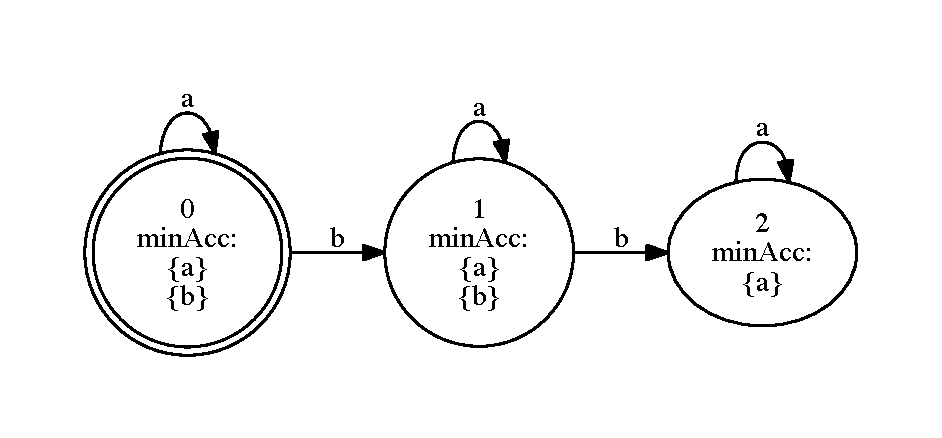
\includegraphics[trim=1.4cm 0cm 0cm 0cm,clip,width=1.1\textwidth]{theorem5p.pdf}
\end{minipage}
\hfill
\begin{minipage}{.55\textwidth}
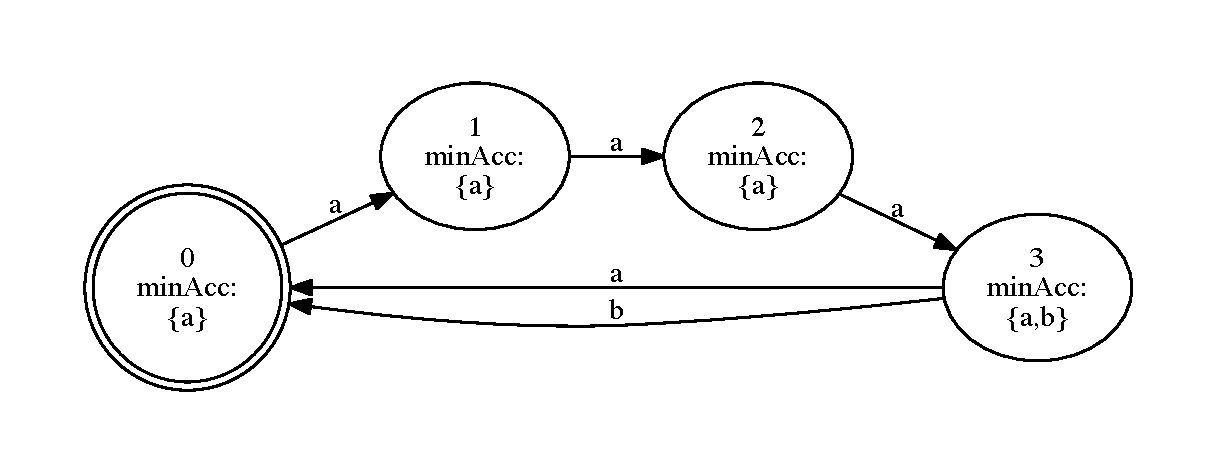
\includegraphics[trim=1.4cm 0cm 0cm 0cm,clip,width=1.1\textwidth]{theorem5q.pdf}
\end{minipage}
\caption{Transition graphs of $P$ (left) and $Q$ (right) from Example~\ref{ex:pq}
 for $p=3$ and $q=4$.}
\label{fig:examplepq}
\end{center}
\end{figure}

% ----------------------------------------------------------------------------
\begin{theorem}\label{th:maxtracelen}
Let $2\le p,q \in\mathbb{N}$. Then there exists a reference process $P$ and an
implementation process $Q$ with the following properties.
\begin{enumerate}
\item $G(P)$ has $p$ states.
\item $G(Q)$ has $q$ states.
\item $P\not\lessdet_T Q$, and therefore, also $P\not\lessdet_F Q$.
\item $\forall s\in\trc(Q): \#s < pq\implies s\in\trc(P)$.
\item $Q\ conf\ P$.
\end{enumerate}
As a consequence, the upper bound $pq$ for the length of traces to be tested when checking for failures refinement or trace refinement
cannot be reduced without losing the test suite's completeness property.
\end{theorem}
% ----------------------------------------------------------------------------
\begin{proof}
Given $2\le p,q \in\mathbb{N}$, define reference process $P$ and
implementation process $Q$ as in Example~\ref{ex:pq}. It is trivial to see
that $G(P)$ has $p$ nodes and $G(Q)$ has $q$ nodes, so statements 1 and 2 of
the theorem hold. Using regular expression notation, the traces of $P$ can be
specified as
\[
\trc(P) = \prefs\big(  (a^*b)^{p-1}a^* \big),
\]
where $\prefs(M)$ denotes the set of all prefixes of traces in $M\subseteq\Sigma^*$,
including the traces of $M$ themselves.
The traces of $Q$ can be specified by
\[
\trc(Q) = \prefs\big( (a^{q-1}(a|b))^*  \big).
\]
It is easy to see that $\trc(Q)\not\subseteq\trc(P)$; for example, the trace
$(a^{q-1}b)^p$ is in $\trc(Q)\setminus\trc(P)$, because $P$-traces may contain at most $p-1$ $b$-events. This proves statement~3 of the theorem.

Let $s \in\trc(Q)$ be any trace of length $\#s = pq-1$. Then $s$ can be represented
by $s = (a^{q-1}(a|b))^{p-1}a^{q-1} \in \prefs\big( (a^{q-1}(a|b))^*  \big)$.
Then $s$ is also an element of $\trc(P)$, because $(a^{q-1}(a|b))^{p-1}a^{q-1}$
is also contained in $\prefs\big(  (a^*b)^{p-1}a^* \big)$: this is easy to see, since
$\prefs\big(  (a^*b)^{p-1}a^* \big)$ contains all finite sequences of $a$-events,
where at most $p-1$ events $b$ have been inserted. This proves statement 4 of the theorem.

To prove statement~5, we observe that the specification of $P$ implies (the
expression $(s\cnt b)$ denotes the number of $b$-events occurring in trace $s$)
\[
\minaccs(P/s) = \left\{
\begin{array}{ll}
\{ \{a\}, \{b\} \} & \text{for all $s\in\trc(P)$ with $(s\cnt b) <p-1$.}
\\
\{ \{a\} \} & \text{for all $s\in\trc(P)$ with $(s\cnt b) = p-1$.}
\end{array}
\right.
\]
and
\[
\minaccs(Q/s) = \left\{
\begin{array}{ll}
\{ \{a\}  \} & \text{for all $s\in\trc(Q)$ with $\#s \neq 0\mod(q-1)$.}
\\
\{ \{a,b\} \} & \text{for all $s\in\trc(P)$ with $\#s = 0\mod(q-1)$.}
\end{array}
\right.
\]
As a  consequence, the minimal acceptance set $A_P = \{a\}$ which is
contained in every $\minaccs(P/s)$ fulfils $A_P \subseteq A_Q$ for
any $A_Q\in\minaccs(Q/s)$, when $s\in\trc(P)\cap \trc(Q)$. Now Lemma~\ref{lemma:tgtrcref},
(\ref{eq:failrefb}) can be applied to conclude that $Q\ conf\ P$.
\xbox
\end{proof}
%
Since Theorem~\ref{th:maxtracelen} just states that a violation of trace
refinement may remain undetected if only traces shorter than $pq$ are checked
during tests, it can also be applied to our trace refinement tests.
Therefore, test suites $\{ U_T(j) \}$ with $j<pq-1$ are not complete. It is
discussed in Section~\ref{sec:conc} how the number of test traces to be
executed by complete test suites for failures or trace refinement can still
be reduced {\it without} reducing the maximal length.

% =================================================================================
